\section{Backend und Persistenz}
\begin{frame}
    \frametitle{Backend und Persistenz}
    \begin{itemize}
        \item In unserem Konzept wird das Dokument nur von Clients bearbeitet.
        \item Das Backend hat nur die Aufgabe den State des Dokuments zu speichern und neuen Clients zur Verfügung zu stellen.
        \item Es hört - wie alle Clients - auf der Message Queue mit und schreibt alle State Änderungen in eine MongoDB.
    \end{itemize}
    \centering
    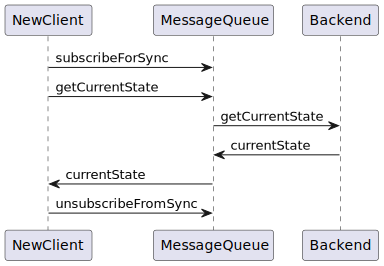
\includegraphics[height=5cm]{media/getStateFromBackend}\label{fig:Get State from Backend Diagramm}
\end{frame}
